\section*{Appendix A}

\subsection*{A.1.1\ \ Mérendő mennyiségek adatai}

{\centering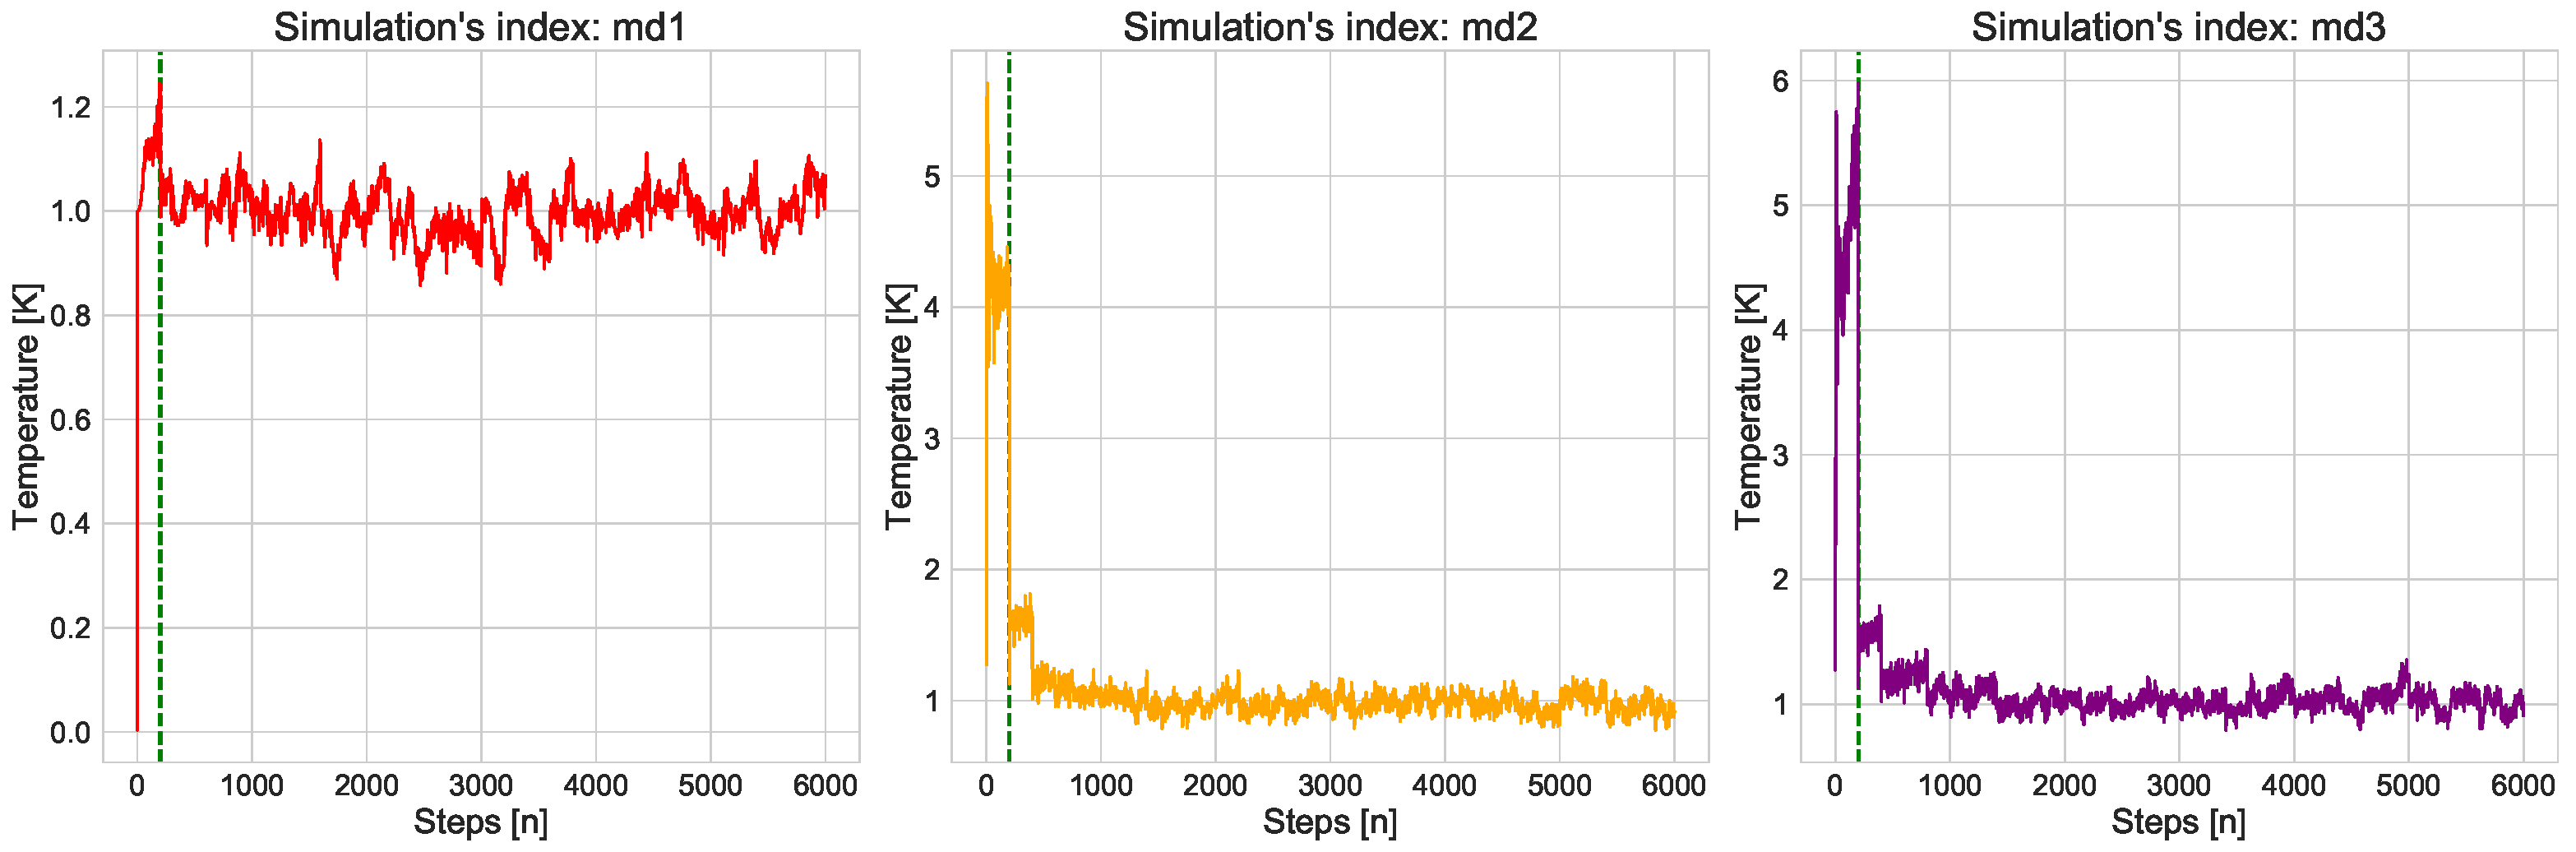
\includegraphics[width=\textwidth]{images/instantaneous_temperatures.pdf}}
\captionof{figure}{Pillanatnyi hőmérsékletek zárt rendszerben, $N = 64$ részecske esetén} \label{fig:1}
\hfill \break \break
{\centering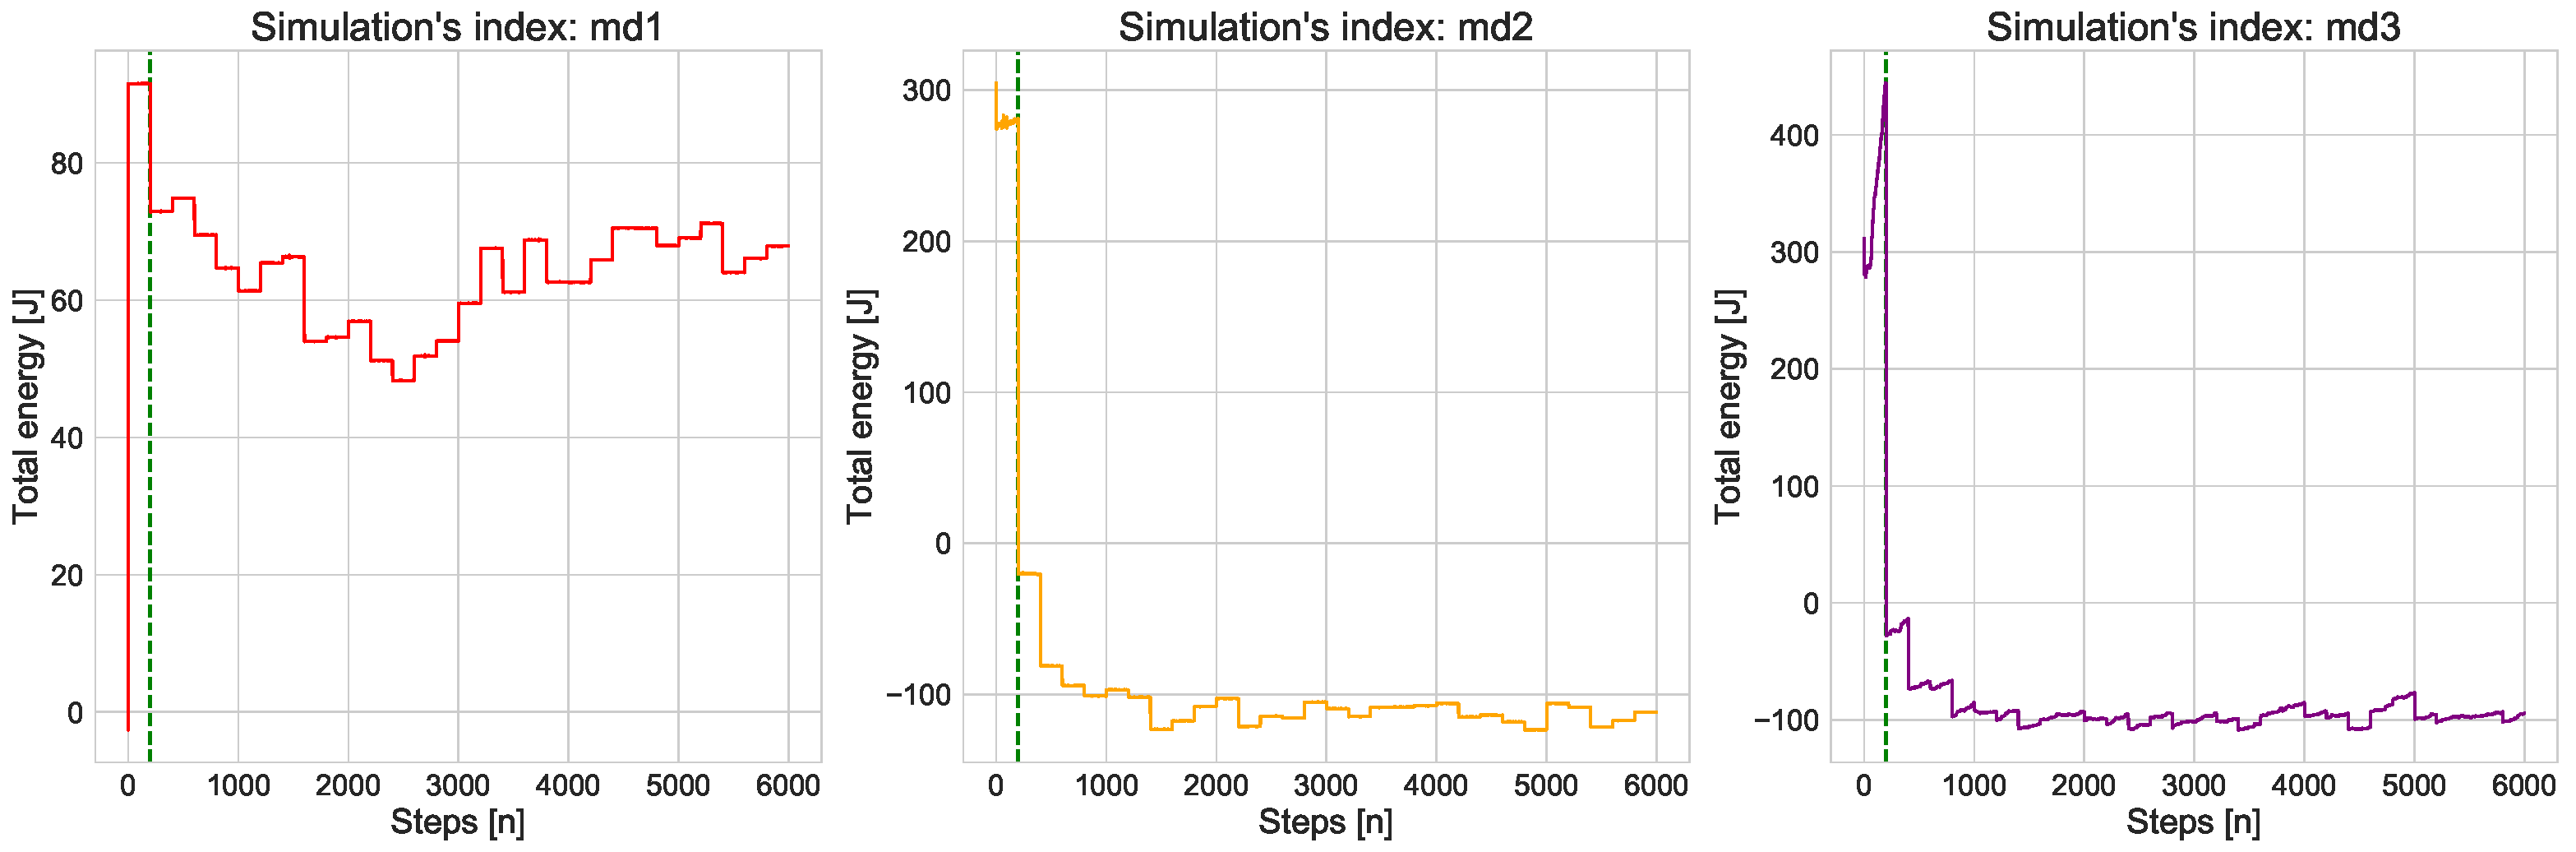
\includegraphics[width=\textwidth]{images/total_energy.pdf}}
\captionof{figure}{A zárt rendszerben teljes energiája $N = 64$ részecske esetén} \label{fig:2}
\hfill \break \break
{\centering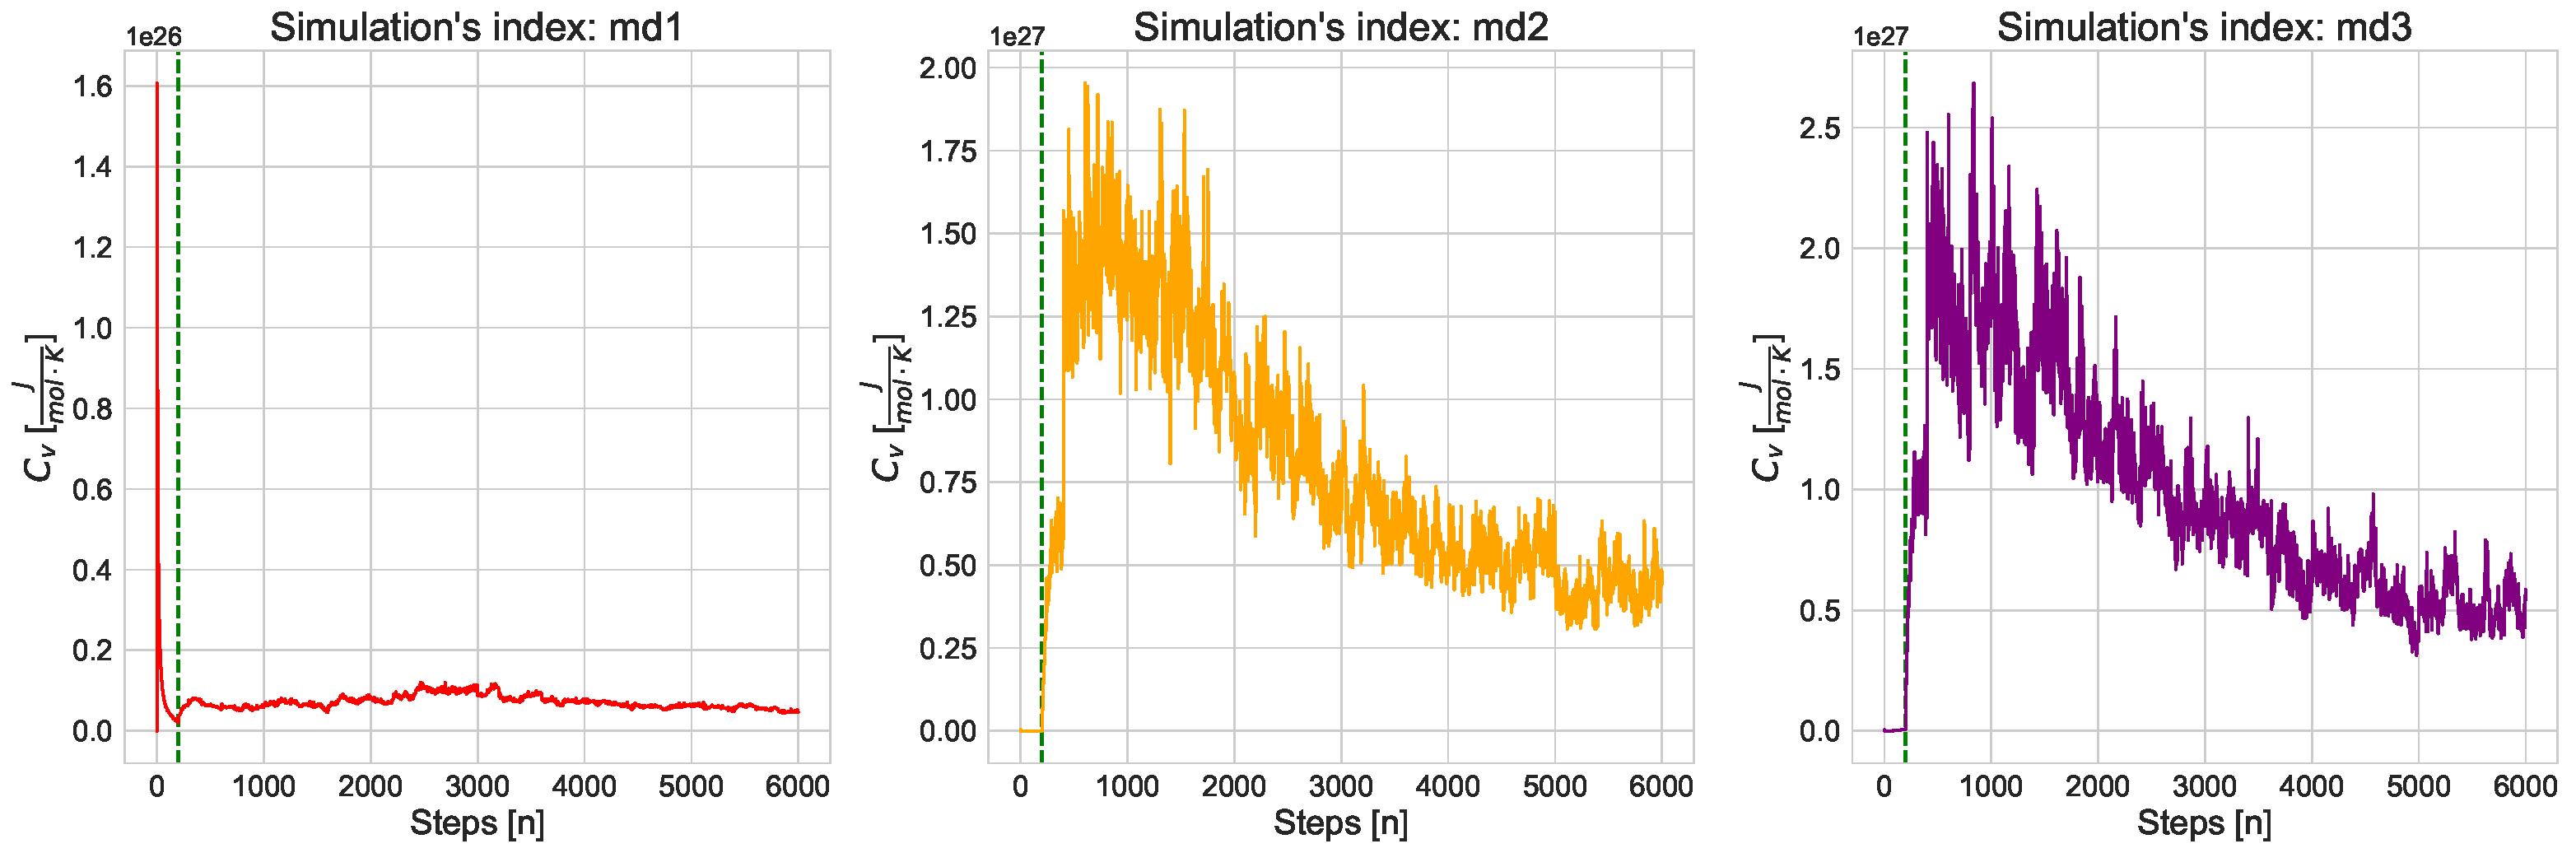
\includegraphics[width=\textwidth]{images/heat_capacity.pdf}}
\captionof{figure}{A zárt rendszerben mért moláris hőkapacitás $N = 64$ részecske esetén} \label{fig:3}
\hfill \break \break
{\centering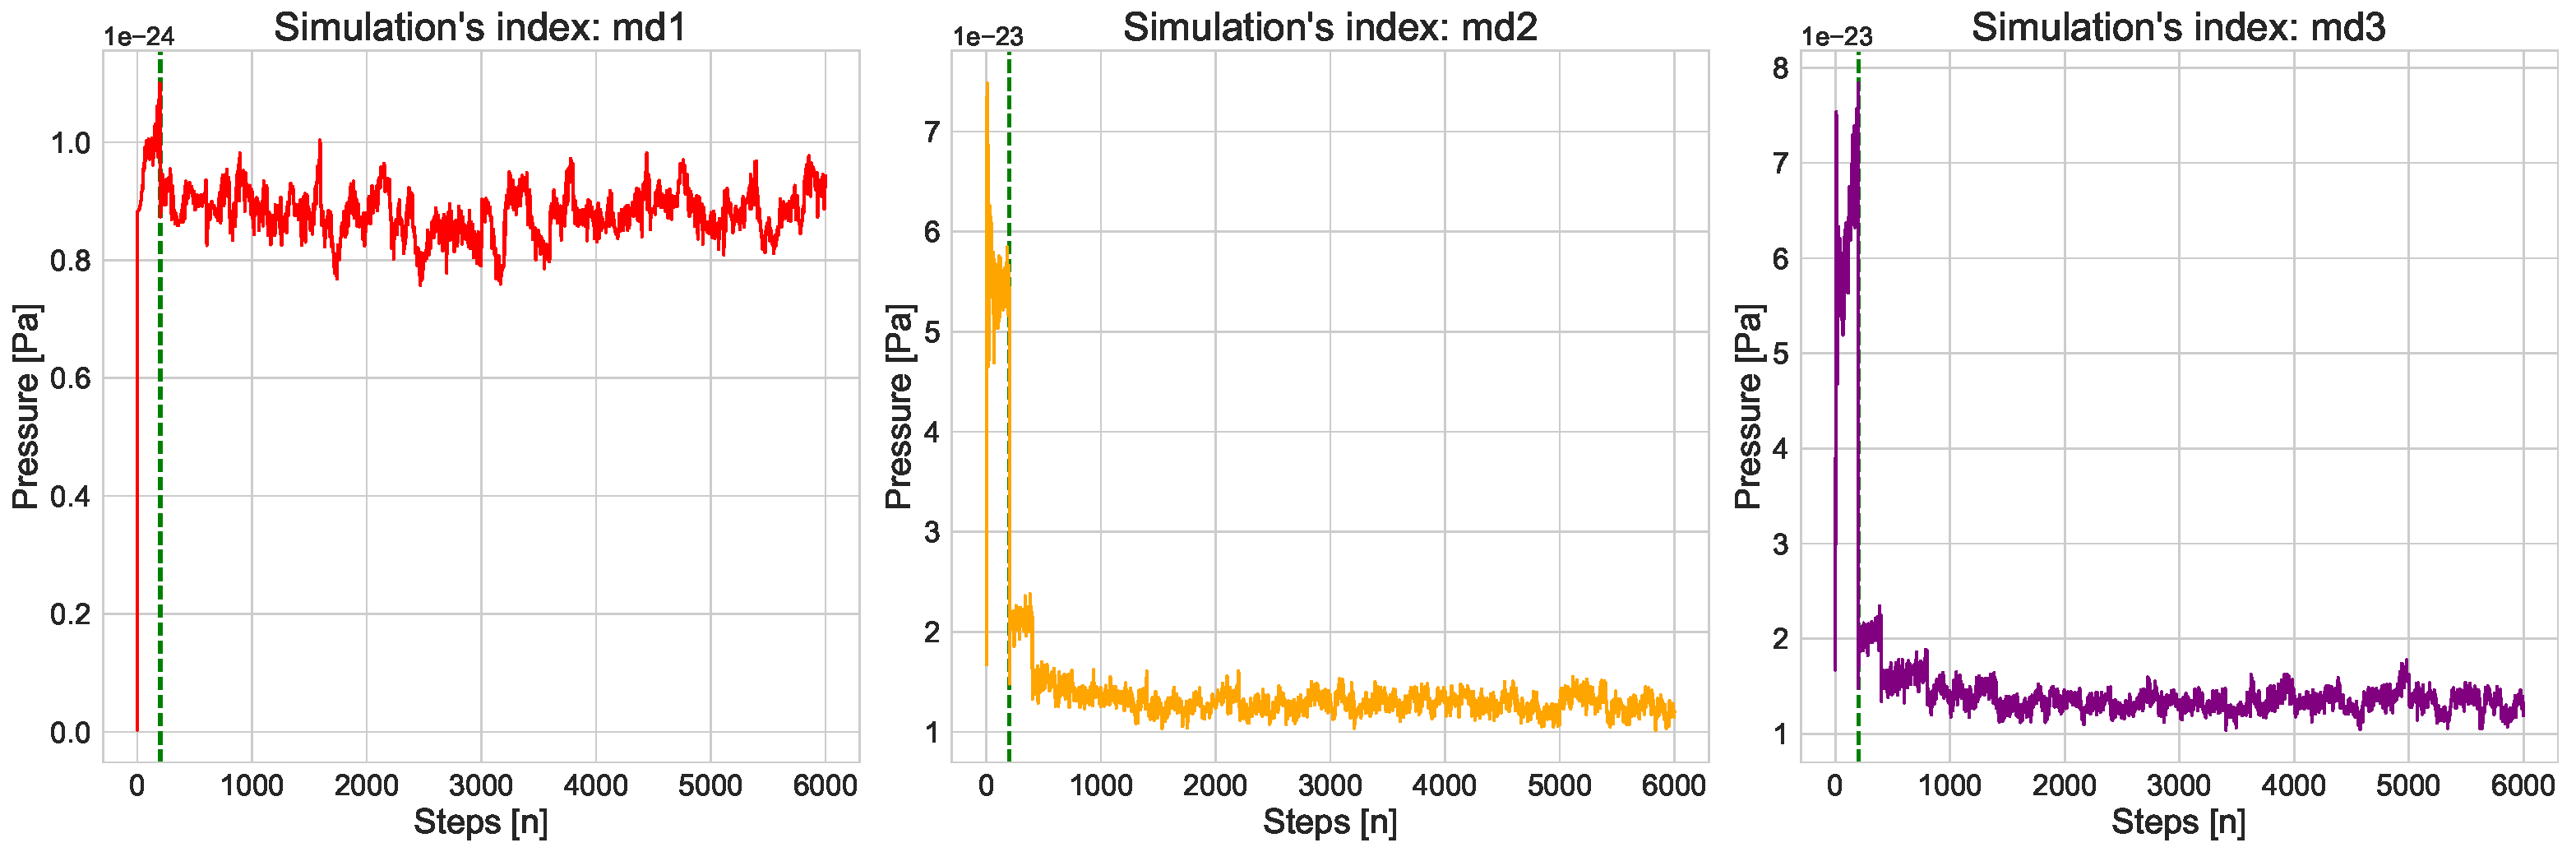
\includegraphics[width=\textwidth]{images/P.pdf}}
\captionof{figure}{A zárt rendszer nyomása $N = 64$ részecske esetén} \label{fig:4}

\newpage

{\centering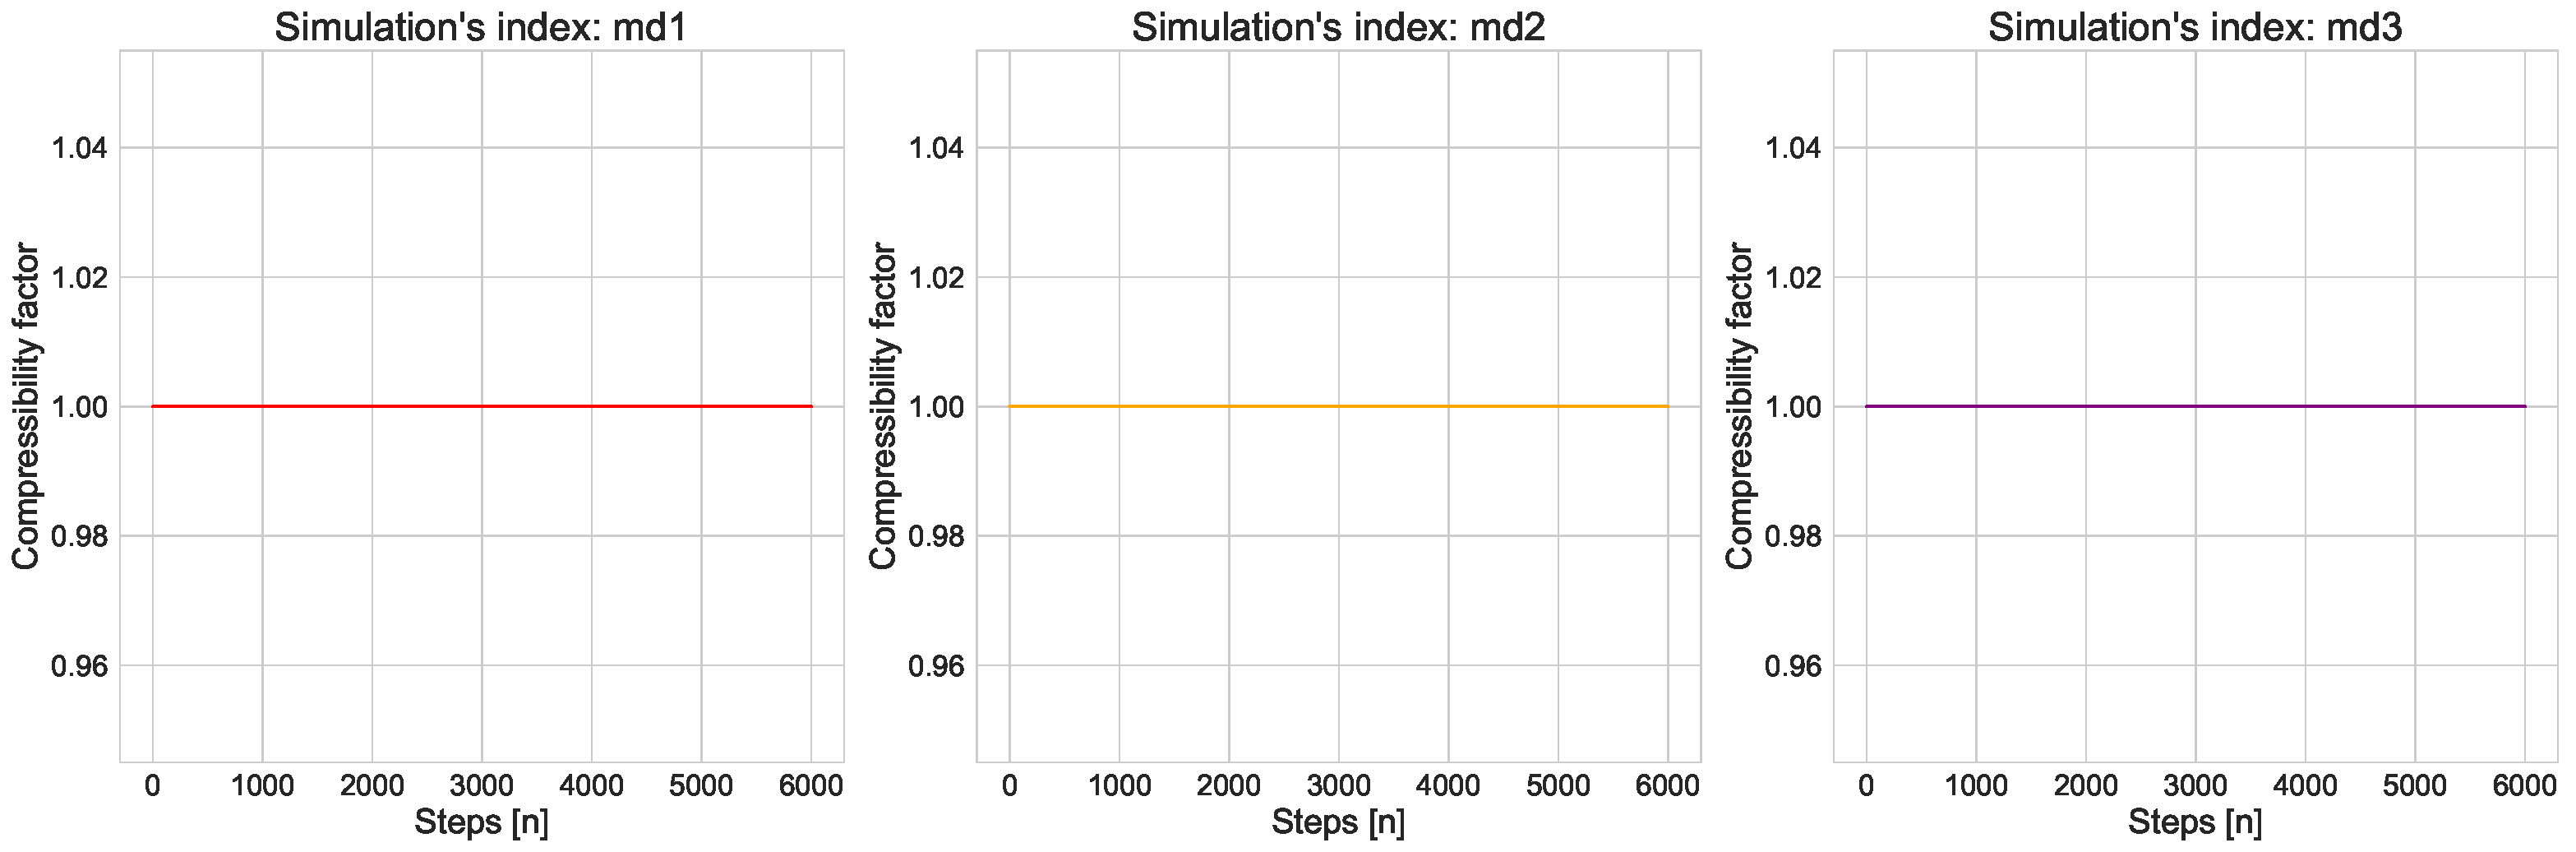
\includegraphics[width=\textwidth]{images/Z.pdf}}
\captionof{figure}{A zárt rendszer kompressziós együtthatója $N = 64$ részecske esetén} \label{fig:5}

\newpage

\subsection*{A.1.2\ \ Futásidők}

{\centering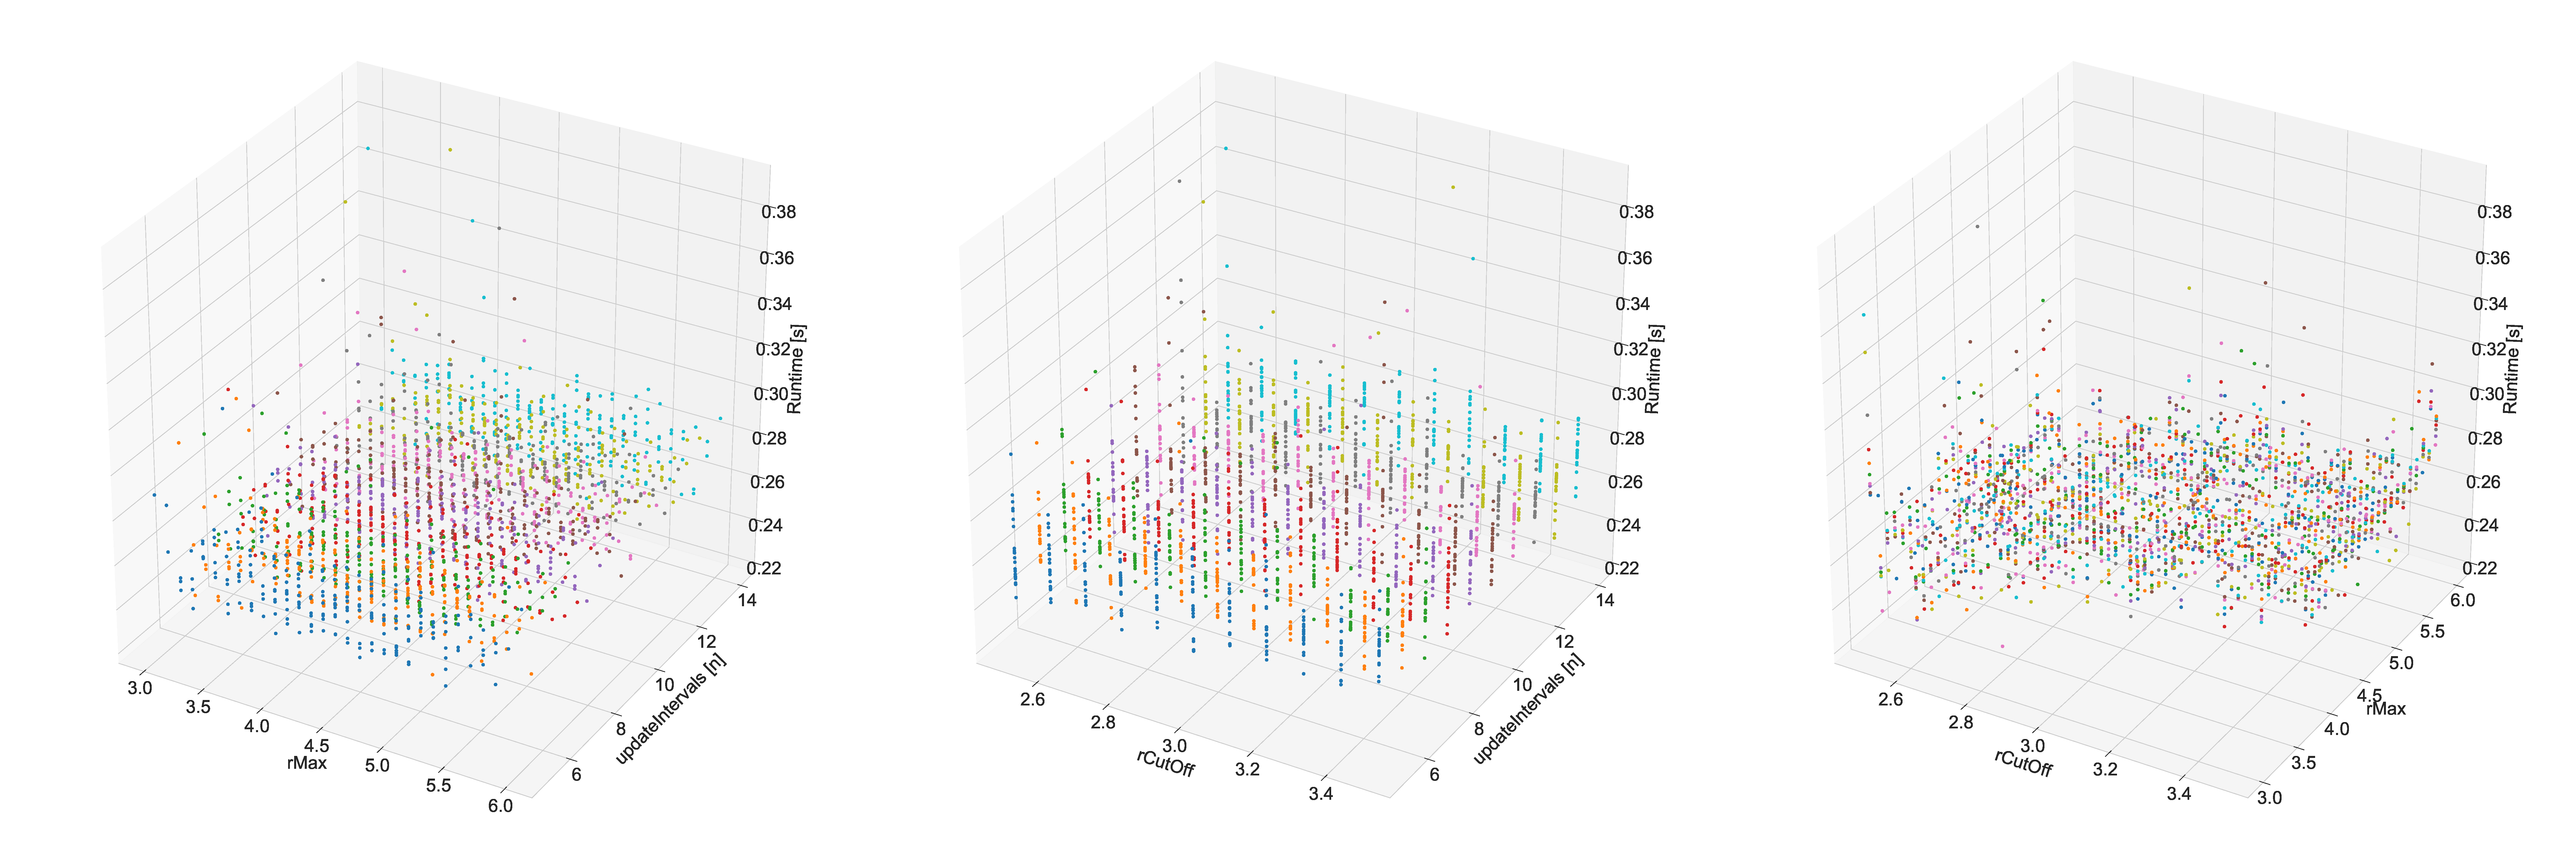
\includegraphics[width=\textwidth]{images/runtime_full_md3.pdf}}
\captionof{figure}{A futásidők teljes 4D terének 3D projekciói. Az azonos szimulációk mindhárom képen azonos színekkel vannak jelölve.\\Bal szélső ábra: Az egyes szimulációk futásideje az \texttt{rMax} és az \texttt{updateInterval} függvényében\\Középső ábra: A futásidők az \texttt{rCutOff} és \texttt{updateInterval} függvényében\\Jobb szélső ábra: A futásidők az \texttt{rCutOff} és \texttt{rMax} függvényében}
\hfill \break \break